\documentclass[10pt]{book}
\usepackage[sectionbib]{natbib}
\usepackage{array,epsfig,fancyhdr,rotating}
\usepackage[driverfallback=dvipdfm]{hyperref}
%%%%%%%%%%%%%%%%%%%%%%%%%%%%%%%%%%%%%%%%%%%%%%%%%%%%%%%%%%%%%%%%%%%%%%%%%%%%%%%%%%%%%%%%%%%%%%%%%%%%%%%%%%%%%%%%%%%%%%%%%%%%

\textwidth=31.9pc
\textheight=46.5pc
\oddsidemargin=1pc
\evensidemargin=1pc
\headsep=15pt
%\headheight=.2cm
\topmargin=.6cm
\parindent=1.7pc
\parskip=0pt


\usepackage{amsmath}
\usepackage{amssymb}
\usepackage{amsfonts}
\usepackage{amsthm}
\usepackage[export]{adjustbox}

\setcounter{page}{1}
\newtheorem{theorem}{Theorem}
\newtheorem{lemma}{Lemma}
\newtheorem{corollary}{Corollary}
\newtheorem{proposition}{Proposition}
\theoremstyle{definition}
\newtheorem{definition}{Definition}
%\newtheorem{proof}{Proof}
\newtheorem{example}{Example}
\newtheorem{remark}{Remark}
\pagestyle{fancy}

% Reference labels in the online appendix
\usepackage{xr}
\externaldocument{mdi-ss}

%%%%%%%%%%%%%%%%%%%%%%%%%%%%%%%%%%%%%%%%%%%%%%%%%%%%%%%%%%%%%%%%%%%%%%%%%%%%%%%%%%%%%%%%%%%%%%%%%%%%%%%%%%%%%%%%%%%%%%%%%%%%
\pagestyle{fancy}
\def\n{\noindent}
\lhead[\fancyplain{} \leftmark]{}
\chead[]{}
\rhead[]{\fancyplain{}\rightmark}
\cfoot{}
\renewcommand{\headrulewidth}{0pt}

%%%%%%%%%%%%%%%%%%%%%%%%%%%%%%%%%%%%%%%%%%%%%%%%%%%%%%%%%%%%%%%%%%%%%%%%%%%%%%%%%%%%%%%%%%%%%%%%%%%%%%%%%%%%%%%%%%%%%%%%%%%%
%%%%%%%%%%%%%%%%%%%%%%%%%%%%%%%%%%%%%%%%%%%%%%%%%%%%%%%%%%%%%%%%%%%%%%%%%%%%%%%%%%%%%%%%%%%%%%%%%%%%%%%%%%%%%%%%%%%%%%%%%%%%

\begin{document}
%%%%%%%%%%%%%%%%%%%%%%%%%%%%%%%%%%%%%%%%%%%%%%%%%%%%%%%%%%%%%%%%%%%%%%%%%%%%%%%%%%%%%%%%%%%%%%%%%%%%%%%%%%%%%%%%%%%%%%%%%%%%
%%%%%%%%%%%%%%%%%%%%%%%%%%%%%%%%%%%%%%%%%%%%%%%%%%%%%%%%%%%%%%%%%%%%%%%%%%%%%%%%%%%%%%%%%%%%%%%%%%%%%%%%%%%%%%%%%%%%%%%%%%%%

\renewcommand{\baselinestretch}{2}

\markright{ \hbox{\footnotesize\rm Statistica Sinica: Supplement
%{\footnotesize\bf 24} (201?), 000-000
}\hfill\\[-13pt]
\hbox{\footnotesize\rm
%\href{http://dx.doi.org/10.5705/ss.20??.???}{doi:http://dx.doi.org/10.5705/ss.20??.???}
}\hfill }

\markboth{\hfill{\footnotesize\rm JASON POULOS AND RAFAEL VALLE} \hfill}
{\hfill {\footnotesize\rm MISSING DATA IMPUTATION FOR SUPERVISED CLASSIFICATION} \hfill}

\renewcommand{\thefootnote}{}
$\ $\par \fontsize{12}{14pt plus.8pt minus .6pt}\selectfont

%%%%%%%%%%%%%%%%%%%%%%%%%%%%%%%%%%%%%%%%%%%%%%%%%%%%%%%%%%%%%%%%%%%%%%%%%%%%%%%%%%%%%%%%%%%%%%%%%%%%%%%%%%%%%%%%%%%%%%%%%%%%

 \centerline{\large\bf MISSING DATA IMPUTATION }
\vspace{2pt}
 \centerline{\large\bf FOR SUPERVISED CLASSIFICATION}
%\vspace{2pt}
% \centerline{\large\bf IF THIRD LINE IS NEEDED}
\vspace{.25cm}
% \author{Author(s)}
 \centerline{Jason Poulos and Rafael Valle} \vspace{.4cm} 
\vspace{.4cm}
 \centerline{\it University of California, Berkeley}
\vspace{.55cm}
 \centerline{\bf Supplementary Material}
\vspace{.55cm}
\fontsize{9}{11.5pt plus.8pt minus .6pt}\selectfont
\noindent
This file contains descriptive plots of missing data patterns in the benchmark datasets, a description and plots of Bayesian hyperparameter optimization for training neural networks on the benchmark datasets, and test error plots for classifiers trained on MCAR-perturbed categorical training features. 
\par

\setcounter{section}{0}
\setcounter{equation}{0}
\def\theequation{S\arabic{section}.\arabic{equation}}
\def\thesection{S\arabic{section}}

\fontsize{12}{14pt plus.8pt minus .6pt}\selectfont

\section{Patterns of missing data}

\newpage
\lhead[\footnotesize\thepage\fancyplain{}\leftmark]{}\rhead[]{\fancyplain{}\rightmark\footnotesize\thepage}%Put this line in Page 2

\begin{figure}[h!]
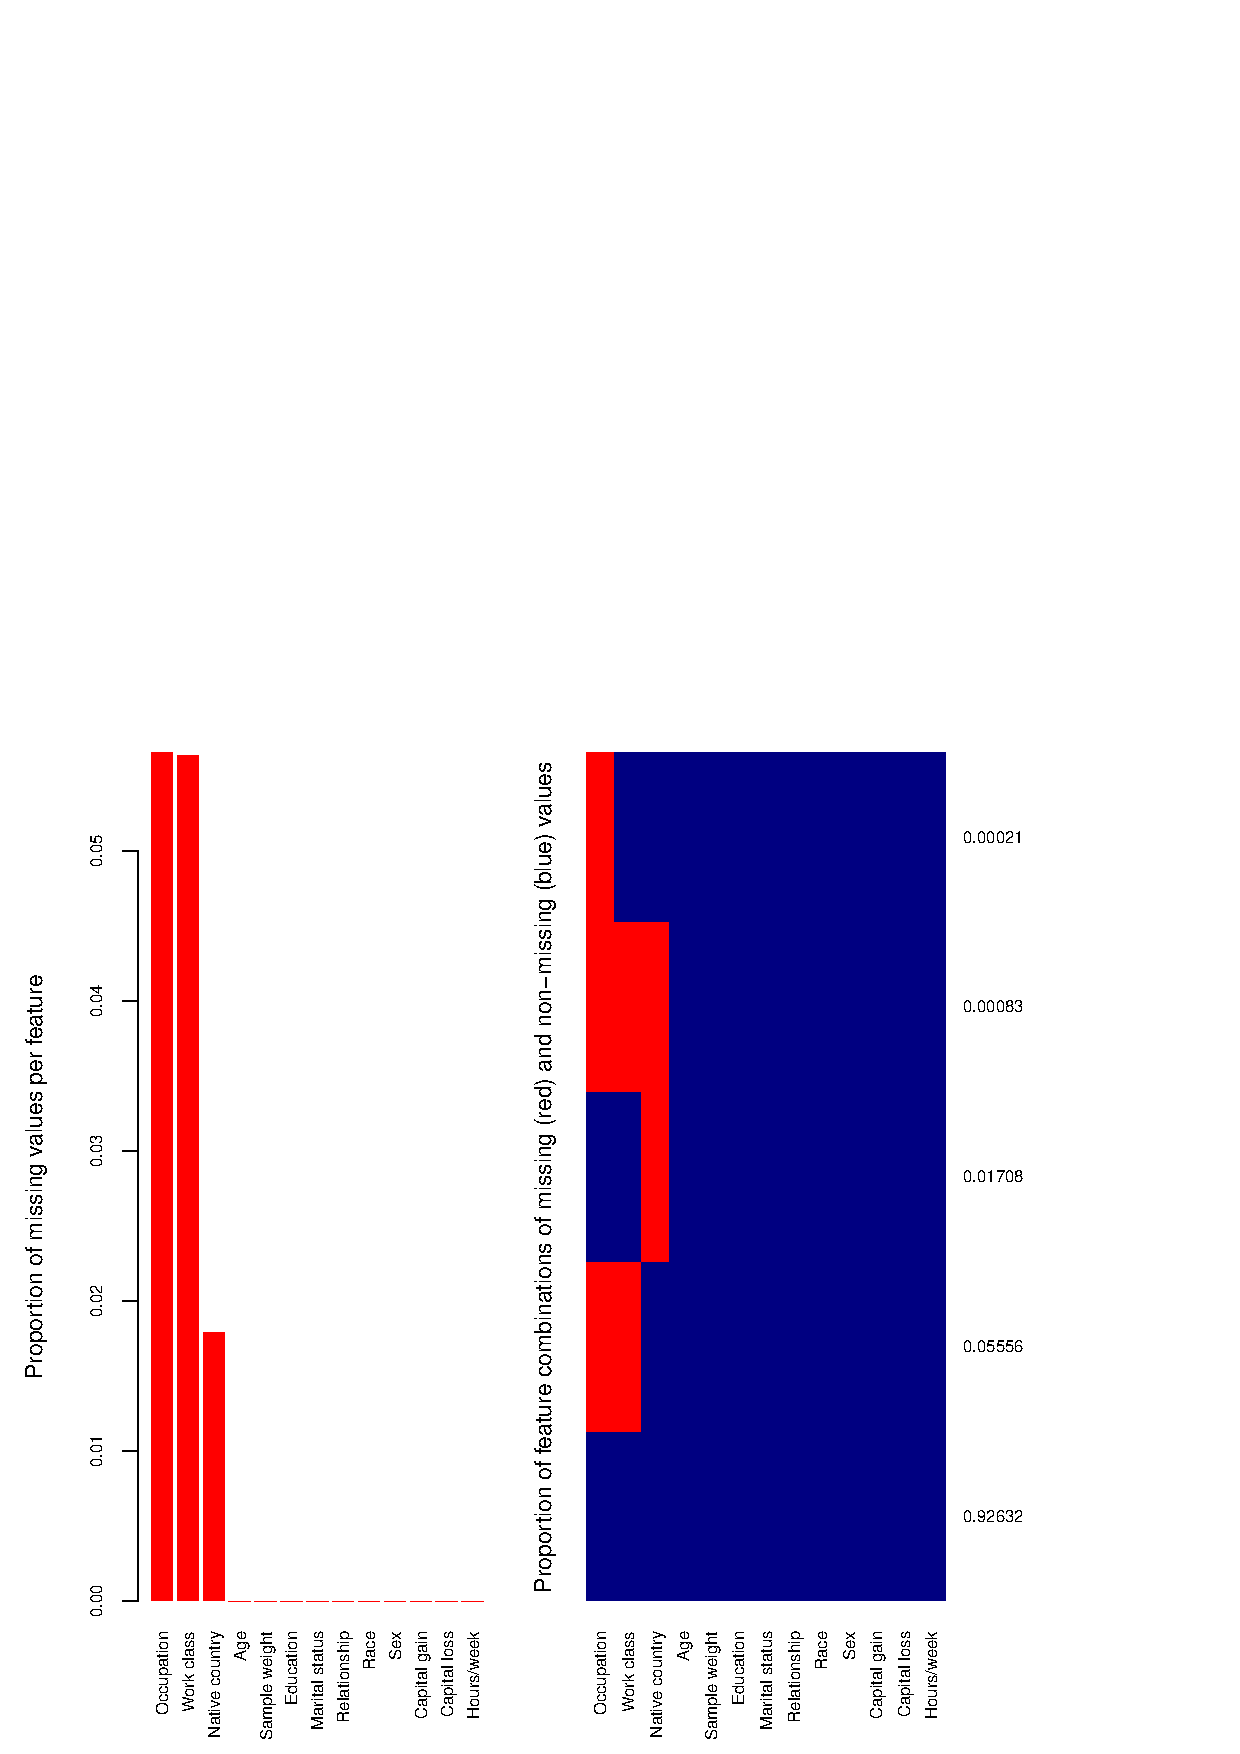
\includegraphics [scale=0.45]{figure/proportion-missing-adult.pdf}\par
\caption{\footnotesize Histogram of proportion of missing values in each feature (Left) of Adult training set and aggregation plot of all existing combinations of missing and non-missing values in the samples (Right).}
 \label{fig:proportion-missing-adult}
\end{figure}

\clearpage
\markboth{\hfill{\footnotesize\rm JASON POULOS AND RAFAEL VALLE} \hfill}
{\hfill {\footnotesize\rm MISSING DATA IMPUTATION FOR SUPERVISED CLASSIFICATION} \hfill}

\begin{figure}[h!]
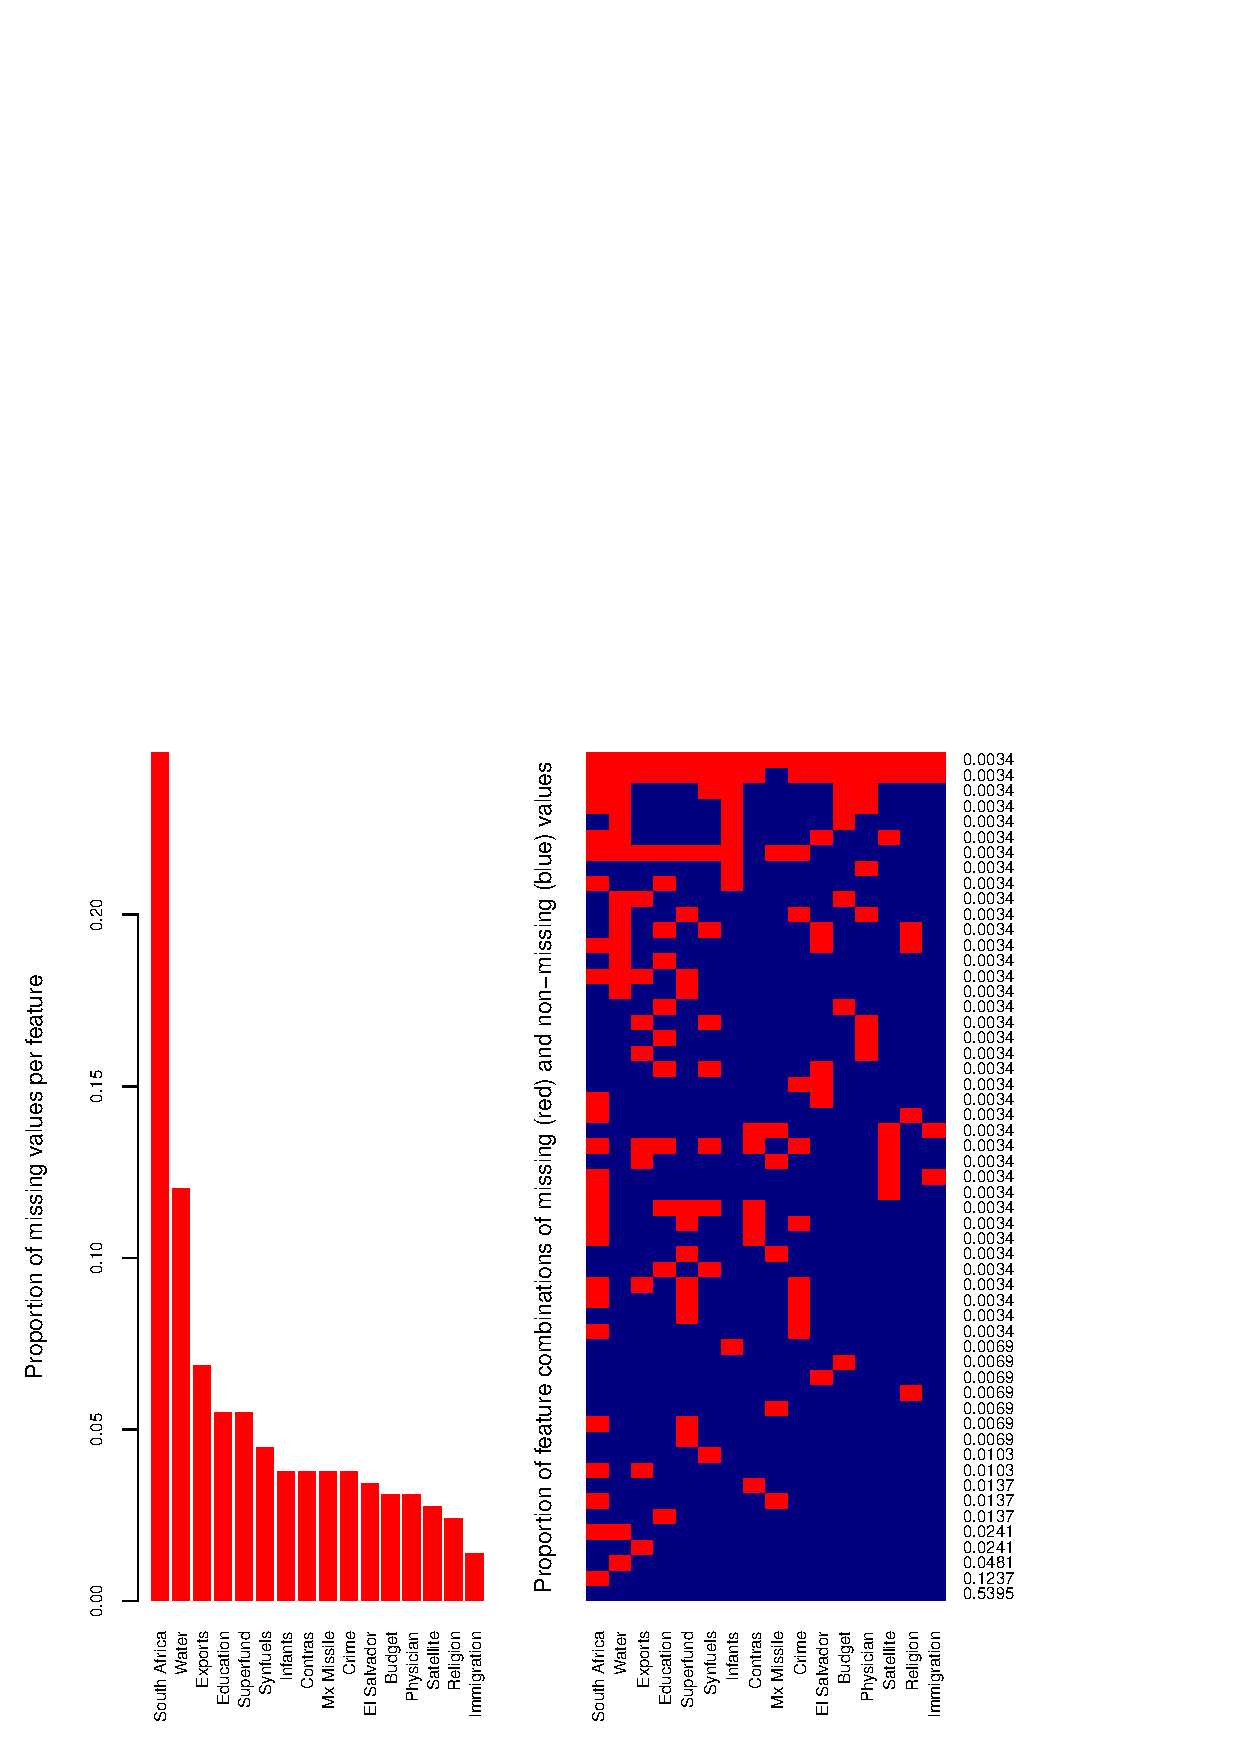
\includegraphics [scale=0.45]{figure/proportion-missing-votes.pdf}\par
\caption{\footnotesize Histogram of proportion of missing values in each feature (Left) of CVRs training set and aggregation plot of all existing combinations of missing and non-missing values in the samples (Right).}
 \label{fig:proportion-missing-votes}
\end{figure}

\clearpage
\markboth{\hfill{\footnotesize\rm JASON POULOS AND RAFAEL VALLE} \hfill}
{\hfill {\footnotesize\rm MISSING DATA IMPUTATION FOR SUPERVISED CLASSIFICATION} \hfill}

\section{Bayesian hyperparameter optimization}
\setcounter{equation}{0}

The goal of Bayesian optimization is to choose a point in the hyperparameter space that appropriately balances information gain and exploitation. Figure \ref{fig:params} shows the exploration of hyperparameter space during Bayesian optimization for both Adult and CVRs datasets. Each circle represents a candidate neural network classifier trained on a differently imputed and perturbed dataset. More circles appear in the plot for CVRs simply due to the fact that the training set is smaller. We see that most of the candidate models use dropout and have an initial learning rate close to the maximum of 0.01. The plurality of candidate models appear to either have momentum (1) or not (0).

\clearpage
\markboth{\hfill{\footnotesize\rm JASON POULOS AND RAFAEL VALLE} \hfill}
{\hfill {\footnotesize\rm MISSING DATA IMPUTATION FOR SUPERVISED CLASSIFICATION} \hfill}

\begin{figure}[h!]
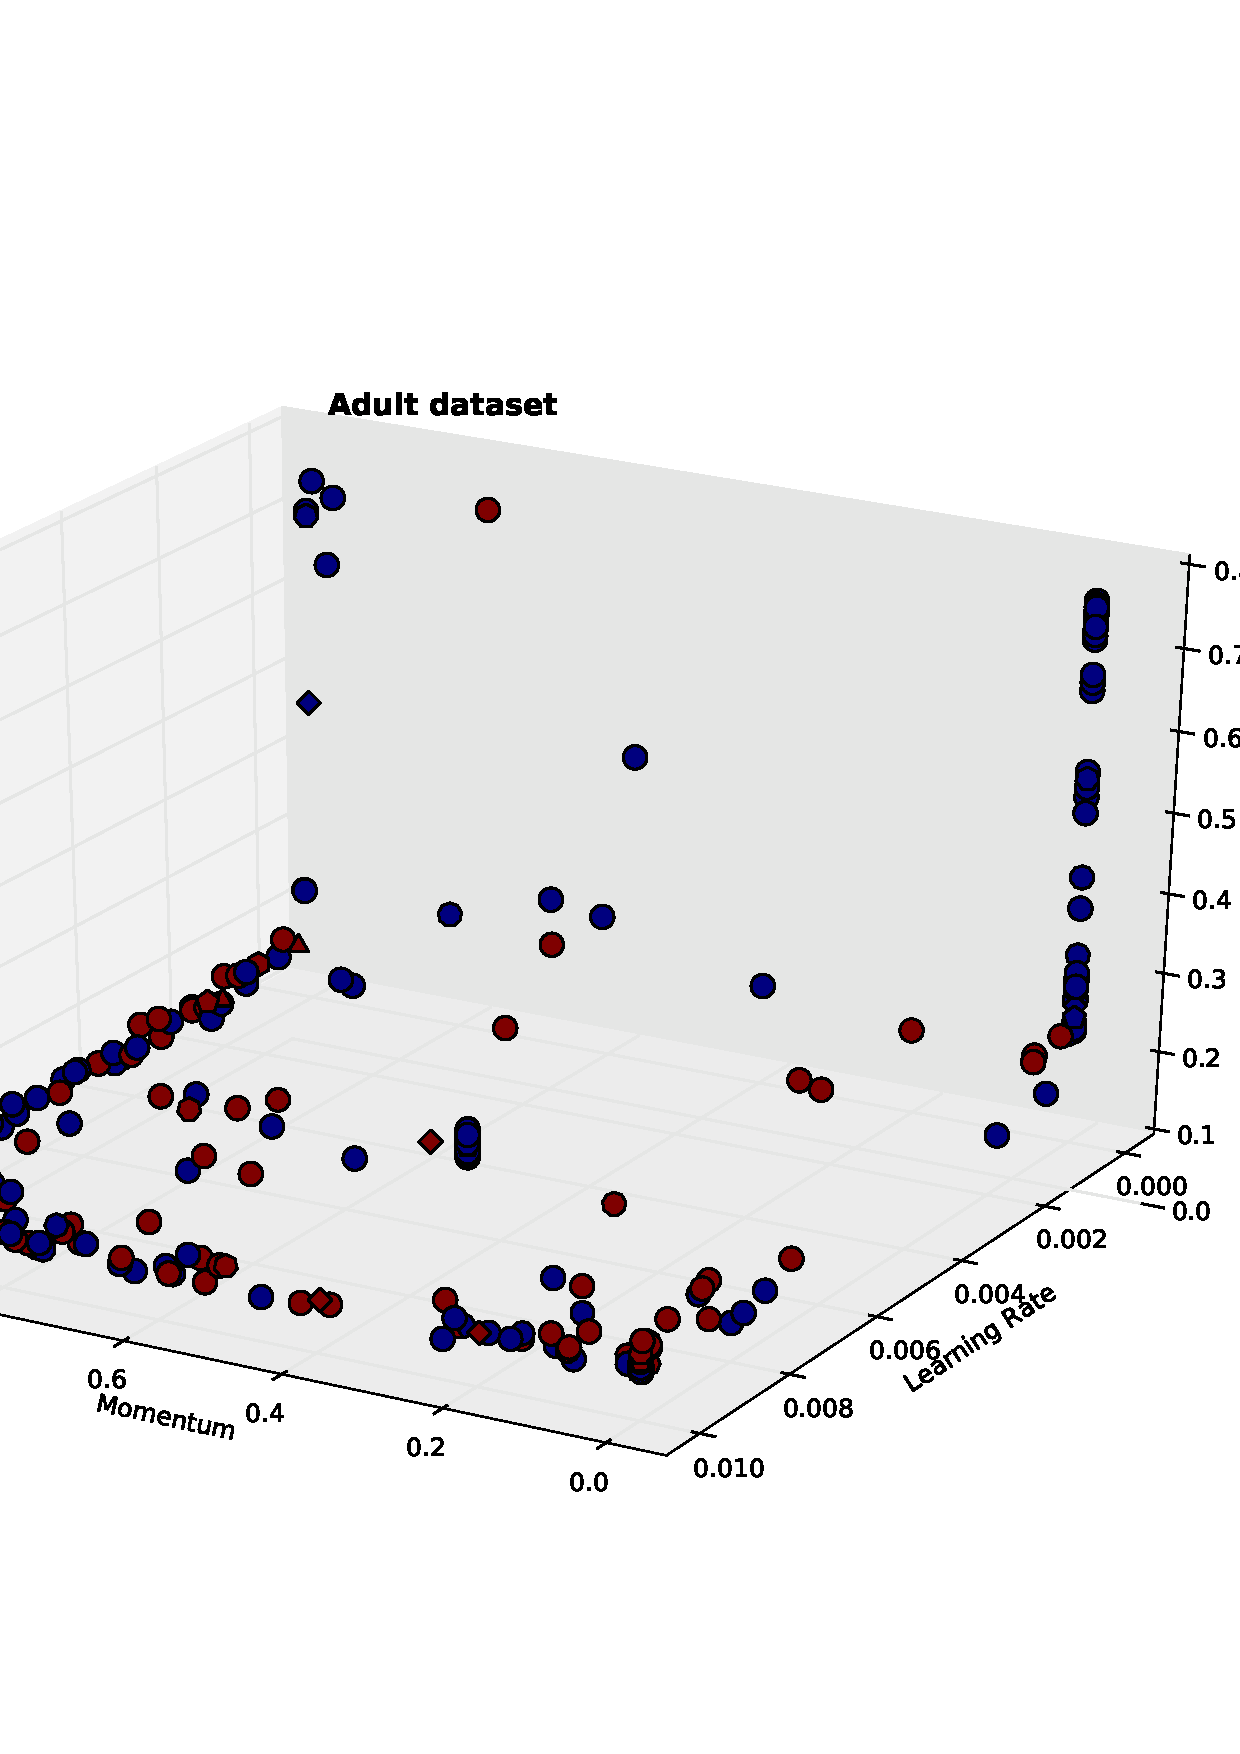
\includegraphics [scale=0.45, center]{../images/params3d_adult.png}\par
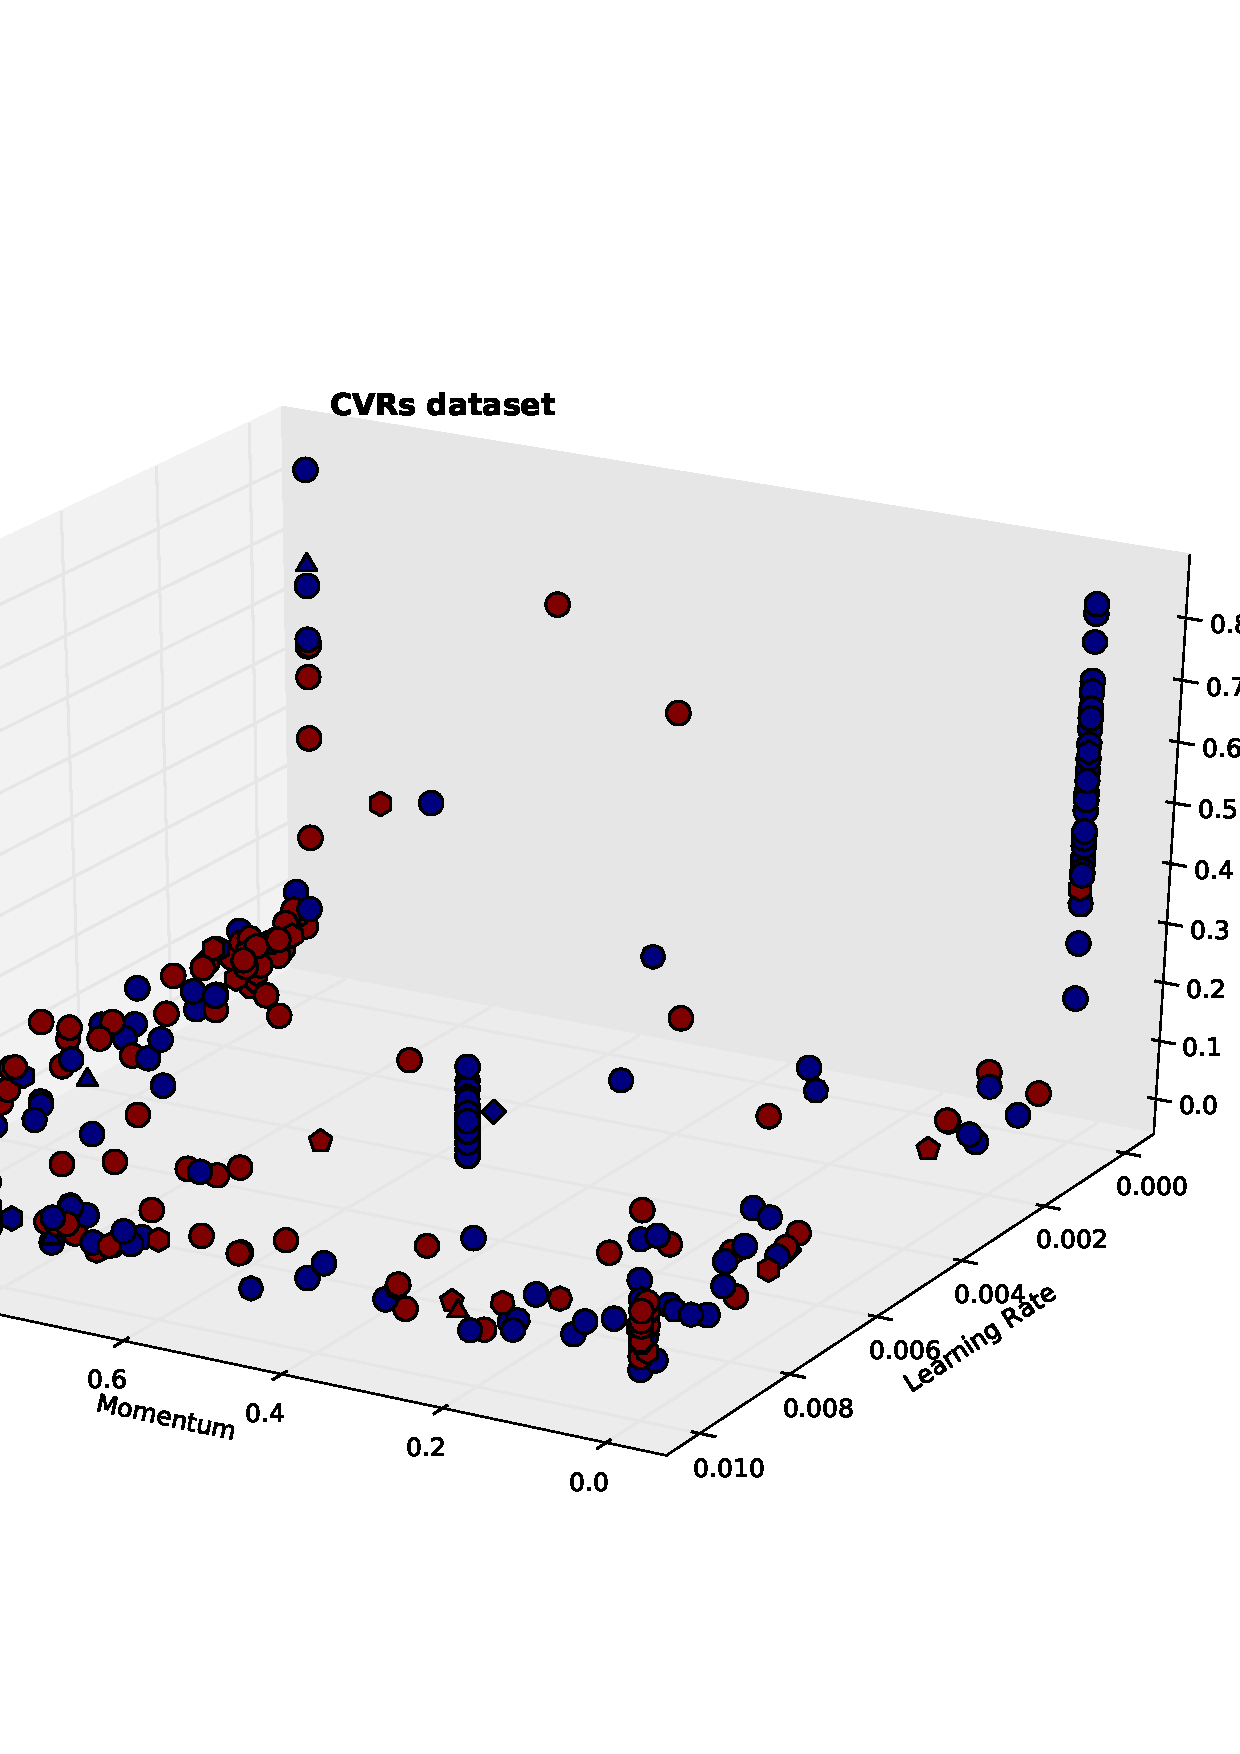
\includegraphics [scale=0.45, center]{../images/params3d_votes.png}\par
\caption{\footnotesize Exploration of hyperparameter space during Bayesian optimization. Each circle represents a candidate neural network classifier trained on a differently imputed and perturbed dataset.}
   \label{fig:params}
\end{figure}

\clearpage
\markboth{\hfill{\footnotesize\rm JASON POULOS AND RAFAEL VALLE} \hfill}
{\hfill {\footnotesize\rm MISSING DATA IMPUTATION FOR SUPERVISED CLASSIFICATION} \hfill}

\section{Results with MCAR perturbation}
\setcounter{equation}{0}

\clearpage
\markboth{\hfill{\footnotesize\rm JASON POULOS AND RAFAEL VALLE} \hfill}
{\hfill {\footnotesize\rm MISSING DATA IMPUTATION FOR SUPERVISED CLASSIFICATION} \hfill}

\begin{figure}[h!]
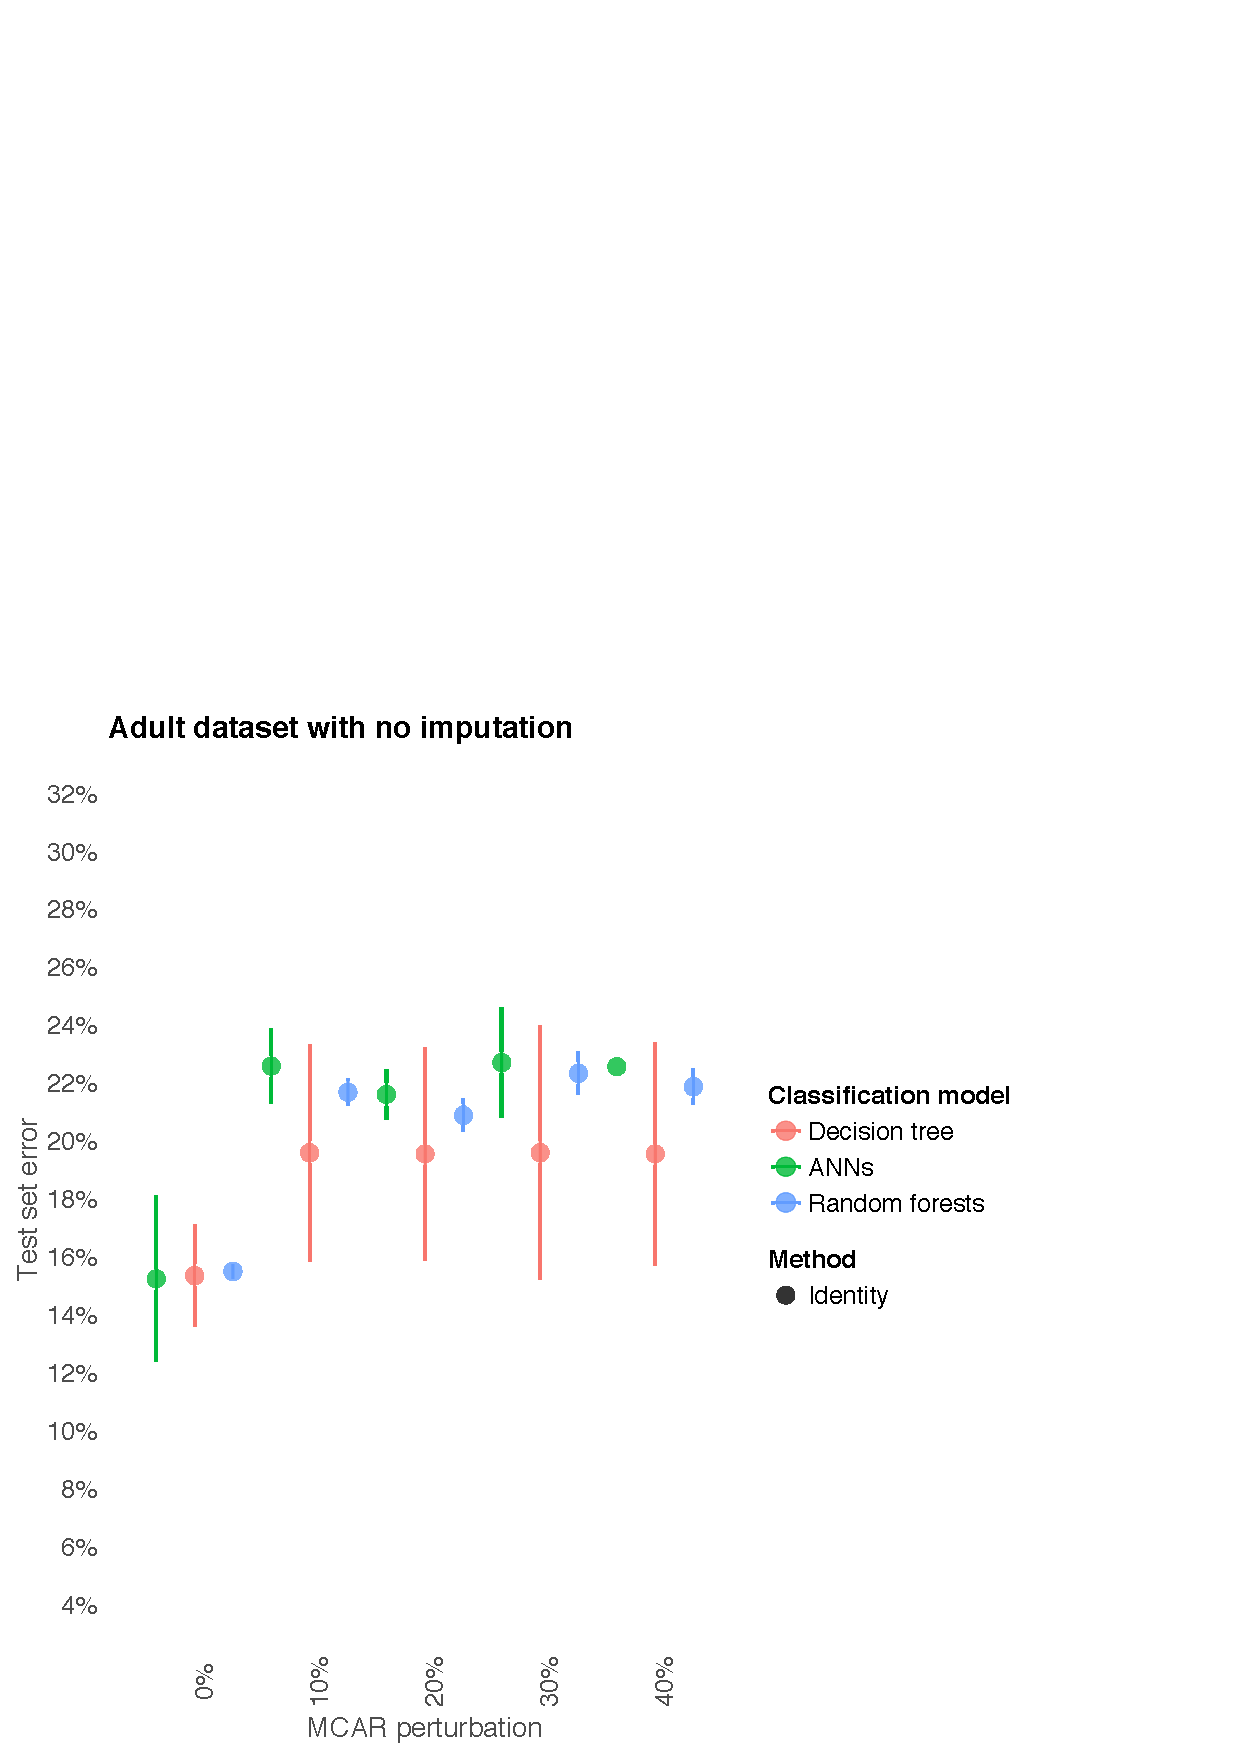
\includegraphics [scale=0.45]{figure/test-errors-adult-no-imp-mcar.pdf}\par
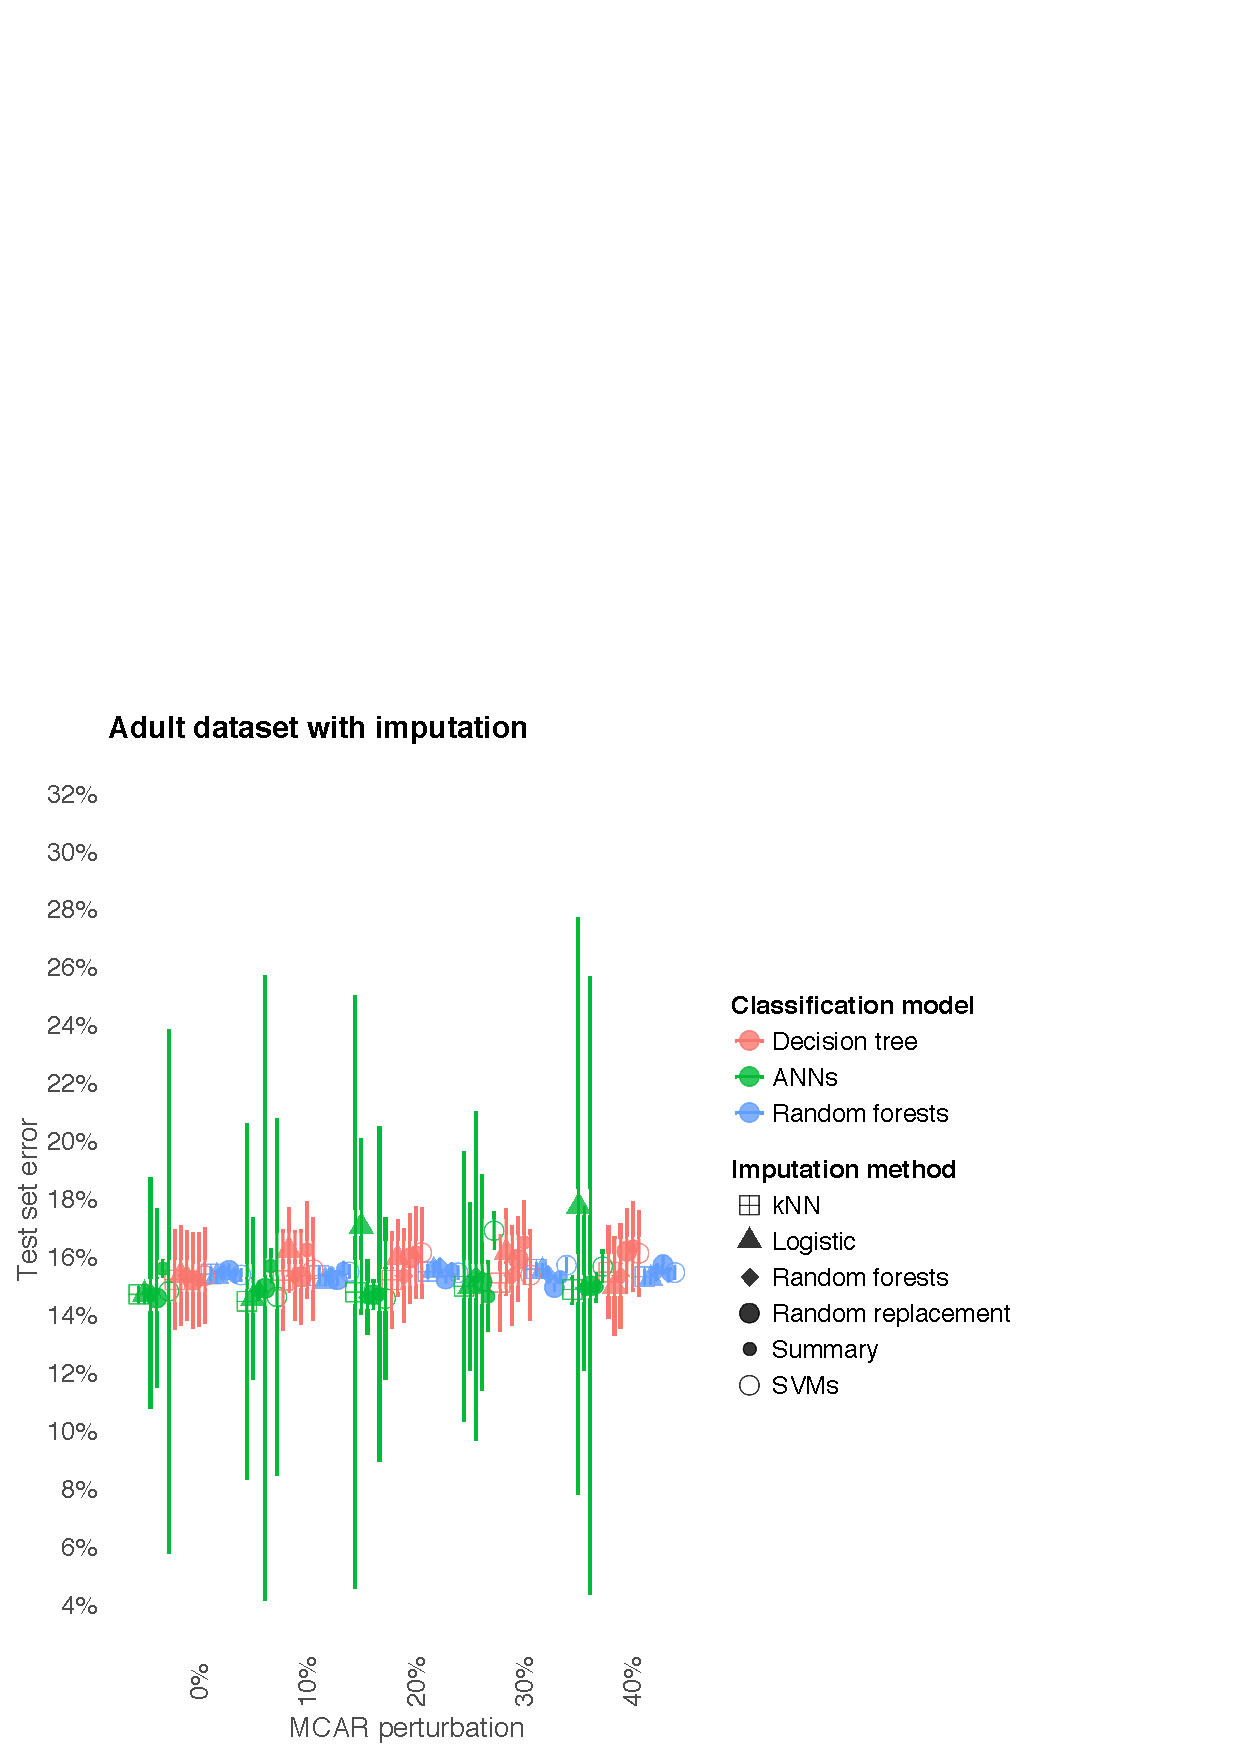
\includegraphics [scale=0.45]{figure/test-errors-adult-imp-mcar.pdf}\par
   \caption{\footnotesize Error rates on the Adult test set with (bottom) and without (top) missing data imputation, for various levels of MCAR-perturbed categorical training features (x-axis). One-hot encoding is used to represent missing data in the absence of imputation. The decision tree and random forests classifiers are trained with maximum depths of 8 and 16, respectively. }
   \label{fig:test-error-adult-mcar}
\end{figure}

\begin{figure}[h!]
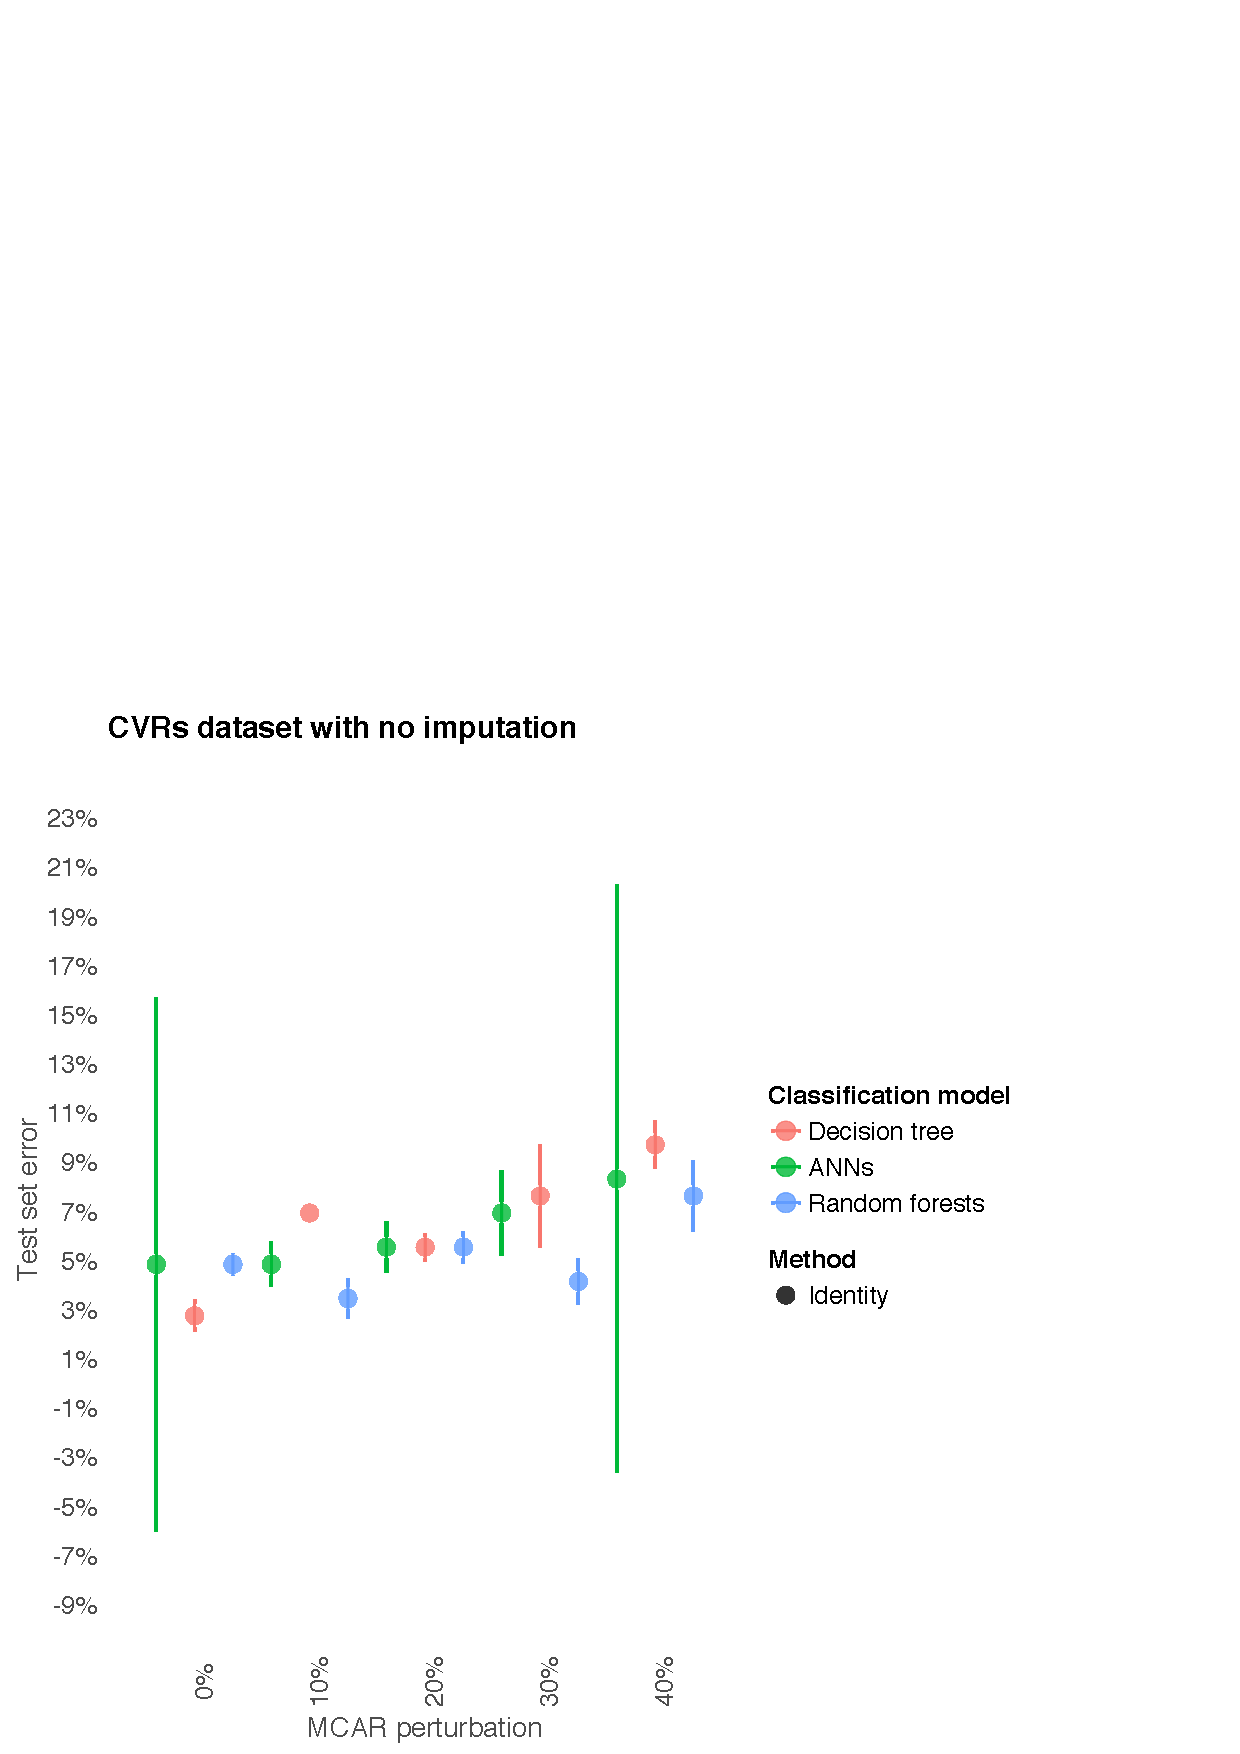
\includegraphics [scale=0.45]{figure/test-errors-votes-no-imp-mcar.pdf}\par
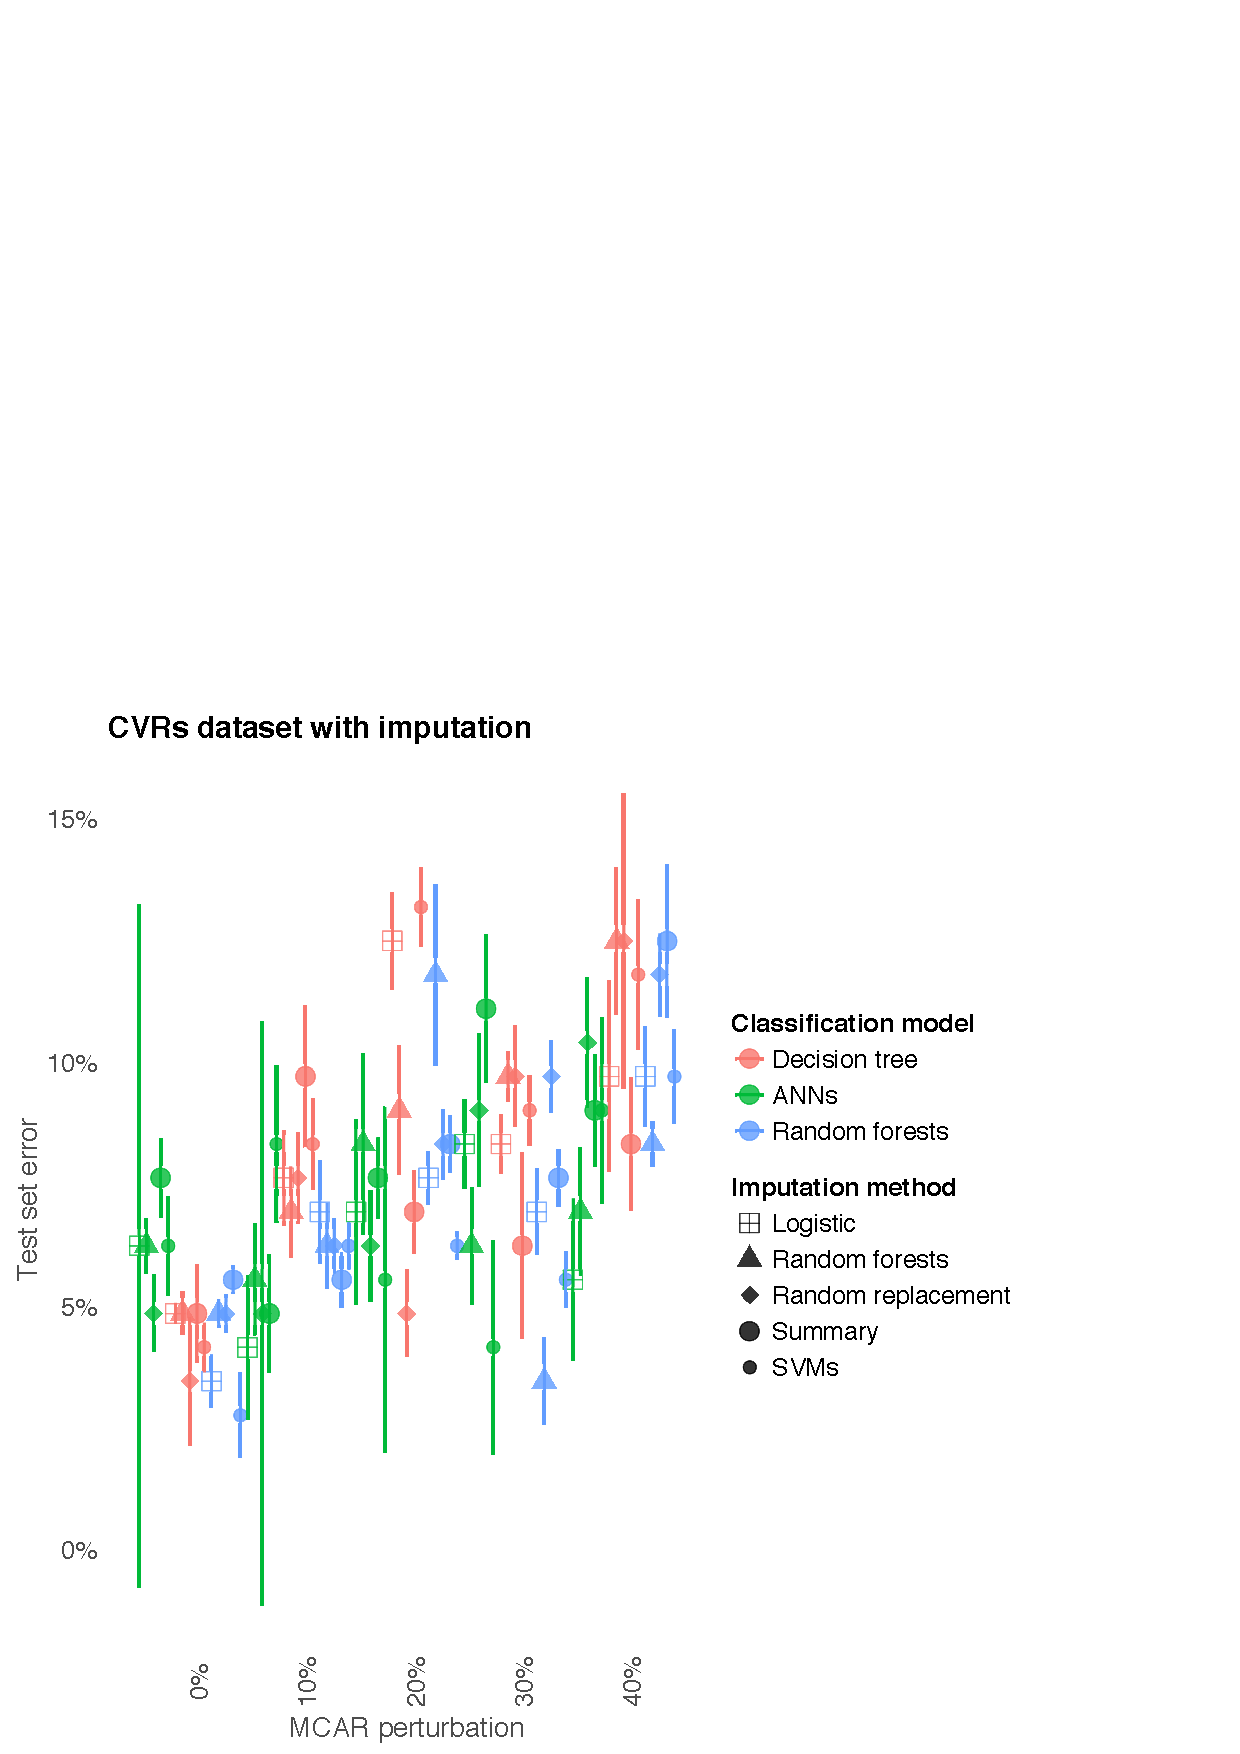
\includegraphics [scale=0.45]{figure/test-errors-votes-imp-mcar.pdf}\par
   \caption{\footnotesize Error rates on the CVRs test set with (bottom) and without (top) missing data imputation. See footnotes for Figure \ref{fig:test-error-adult-mcar}.}
   \label{fig:test-error-votes}
\end{figure}

%\section{Title of section 3}
%\setcounter{equation}{0}
%
%
%\section{Title of section 4}
%\setcounter{equation}{0}

\end{document}
